\documentclass{article}

\usepackage[T1]{fontenc}
\usepackage{graphicx}
\usepackage{fancyhdr}
\pagestyle{fancy}
\fancyhf{}
\lhead{Version 1.3.0}
\rhead{Elliot Oram}
\rfoot{\thepage}


\title{Charades Game Class Diagram}
\author{elo9@aber.ac.uk}

\begin{document}

\maketitle
\tableofcontents

\newpage

\section{Charades Game Class Diagram}
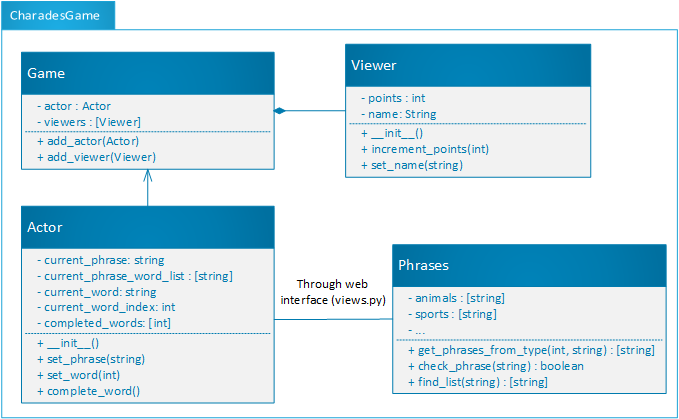
\includegraphics[width=\textwidth]{CharadesGameClass}


\section{Description of Class Diagram}
This is an additional architecture embedded into the Django website. These classes will manage the information that needs to be stored for each player as well as checks to ensure the session has the correct number of players. 

\subsection{Actor}
\subsubsection{Variables}
\begin{itemize}

	\item \textbf{current\_phrase}: Contains the current phrase that the Actor is attempting to act. Type: string.
	
	\item \textbf{current\_phrase\_word\_list}: A list of the words within the phrase. This will be created using the python split() function which separates a string by spaces. This variable will save time having to look up the word each time to display it. Type: string list.

	\item \textbf{current\_word}: Contains the current word in the phrase that is being acted. This is an integer that relates to word. Type: int.
	
	\item \textbf{current\_word\_index}: Holds the current index of the word being acted / guessed. Type: int.
	
	\item \textbf{completed\_words}: A list of integers representing the words that have been completed. A word is completed when it correctly guessed or time has elapsed. Type: int list.
	
	\item \textbf{phrase\_genre}: A string representing the genre of the current phrase e.g. 'Sport'. Type: string.
	
\end{itemize}

\subsubsection{Functions}

\begin{itemize}

	\item \textbf{\_\_init\_\_}: Resets the variables to default values.

	\item \textbf{set\_phrase}: updates the phrase variable with a new string. Updates the phrase word list with a with each word in the phrase. Updates the genre of the phrase.
	
	\item \textbf{set\_word}: updates the word variable with a  new int.
	
	\item \textbf{complete\_word}: adds a word (int) to the completed word list.
	
	\item \textbf{phrase\_complete}: Called when the full phrase has been successfully guessed. The function resets the variables to default values (None, empty lists, ect.)
	
	\item \textbf{phrase\_ready}: Function is linked to the the API usage. Return True when the phrase/word is in a guessable state (phrase selected is True, word selected is True).

\end{itemize}


\subsection{Viewer}
\subsubsection{Variables}

\begin{itemize}
	\item \textbf{points}: The number of points accumulated by the viewer. Type: int.

	\item \textbf{viewer\_number}: Single digit integer used to identify the viewer. This is also stored client side. Type: int.

\end{itemize}

\subsubsection{Functions}

\begin{itemize}

	\item \textbf{\_\_init\_\_}: Resets the variables to default values.

	\item \textbf{increment\_points}: increase the points variable by an integer.
	
\end{itemize}

\subsection{Game}
\subsubsection{Variables}
\begin{itemize}
	\item \textbf{actor}: The actor in the game. (There is only one actor per game. Type: Actor
	
	\item \textbf{viewers}: A list of the viewers in the game. Type: Viewer list.
	
	\item \textbf{current\_correct\_guess}: defaults to None. Hold the current correct guess made by a viewer from the guess interface. Type: String.
	
	\item \textbf{current\_correct\_guess\_type}: defaults to None. Hold the type of guess made by the viewer that was correct ('Word'/'Phrase'). Type: String. 
	
	\item \textbf{winning\_viewer\_number}: Holds the viewer number of the viewer that made the correct guess. This is used for adding points and for reference on the waiting for actor screen.
	
\end{itemize}

\subsubsection{Functions}
\begin{itemize}

	\item \textbf{add\_actor}: Updates the actor variable with a new Actor.
	
	\item \textbf{add\_viewer}: Adds a Viewer to the viewer list variable. There will be a check to ensure the same viewer is not being added again as well as ensure the maximum number of viewers is not exceeded.
	
	\item \textbf{lookup\_viewer}: Looks up the viewer in the viewers list using the viewer\_number to identify them. Returns Viewer.
	
	\item \textbf{get\_viewer\_position}: Looks up the viewers score and their position relative to other viewers in the session. Returns a string for their position (1st, 2nd, ect...).
	
	\item \textbf{set\_guess\_type}: Takes a boolean to represent if the guess type is for the phrase (True) or the word (False).
	
	\item \textbf{set\_guess}: Sets the current correct guess and verify that the guess is correct. The Function will assume a guess type if not already set (is None).
	
	\item \textbf{reset\_guess\_state}: Resets the current\_correct\_guess variables to the default values of None.
	
\end{itemize}

\subsection{Phrases}
\subsubsection{Variables}
\begin{itemize}

	\item \textbf{animals}: All phrases that are animals that can be acted. Type: string list.
	
	\item \textbf{sports}: All phrases that are sports that can be acted. Type: string list.
	
\end{itemize}

\subsubsection{Functions}
\begin{itemize}
	
	\item \textbf{get\_phrase\_from\_type}: A function that get a number of phrases from a type (string list of phrases). The int is the number to retrieve, the string is the type to get. The string are returned in a string list from the function. The function will raise a RuntimeError if the type is unknown (this will be handled neatly in the web interface upon access).
	
	\item \textbf{check\_phrase}: Ensures that a string is present in one of the lists of phrases. This is done by concatenating all the lists and checking the input string is present. Returns a string of the name of the list that the string is present in or False if the string could not be found.
	
	\item \textbf{find\_list}: Takes a string input and return the relevant list matching that string. This is used as a private function for the get\_phrase\_from\_type function.
	
\end{itemize}

\end{document}